\documentclass[12pt,a4paper]{article}
\usepackage[utf8]{inputenc}
\usepackage[T1]{fontenc}
\usepackage[spanish,es-nodecimaldot]{babel}
\usepackage{amsmath,amssymb}
\usepackage{graphicx}
\usepackage{float}
\usepackage{hyperref}
\usepackage{bookmark}
\usepackage{tikz}
\usepackage{geometry}
\usepackage{array}
\usepackage{longtable}
\usepackage{booktabs}
\usepackage{caption}
\usepackage{fancyhdr}
\geometry{left=2.5cm,right=2.5cm,top=2.5cm,bottom=2.5cm}
\setlength{\headheight}{15pt}
\pagestyle{fancy}
\fancyhf{}
\lhead{Trabajo Práctico N\ensuremath{^\circ} 4}
\rhead{Síntesis de Redes Activas}
\cfoot{\thepage}
\captionsetup[figure]{labelfont=bf}
\begin{document}
\begin{titlepage}
\thispagestyle{empty}

\begin{tikzpicture}[remember picture,overlay]
    \node[opacity=0.14,anchor=center] at (current page.center)
        {
\includegraphics[width=0.92\paperwidth]{media/decoracion_a.png}};
\end{tikzpicture}

\begin{center}
    \vspace*{0.8cm}
    
\includegraphics[width=0.82\textwidth]{media/unc_fcefyn_logo.png}

    \vspace{0.8cm}
    {\Large Universidad Nacional de Córdoba\par}
    \vspace{0.2cm}
    {\large Facultad de Ciencias Exactas, Físicas y Naturales\par}
    \vspace{0.2cm}
    {\large Cátedra de Síntesis de Redes Activas\par}

    \vspace{1.6cm}
    {\Large \textbf{Trabajo Práctico N\textsuperscript{o} 4}}\par
    \vspace{0.25cm}
    {\Large Amplificadores compuestos VFA-VFA y VFA-CFA}\par

    \vspace{1.8cm}
    \renewcommand{\arraystretch}{1.35}
    \begin{tabular}{p{6.2cm}p{5.5cm}}
        \textbf{Integrantes} & \textbf{DNI} \\
        Bayón, Pablo & 39.402.464 \\
        Godoy, Emiliano & 41.524.015 \\
        Luna, Fernando Valentino & 43.612.136 \\
        Testa, Lisandro Daniel & 43.477.019 \\
    \end{tabular}

    \vspace{1.2cm}
    \begin{tabular}{p{4.2cm}p{7.8cm}}
        \textbf{Docentes} & Prof. Ferreyra, Pablo Alejandro \\
                          & Prof. Reale, César \\
    \end{tabular}

    \vfill
    Córdoba, República Argentina\\
    \today
\end{center}
\end{titlepage}

\tableofcontents
\listoffigures
\newpage
\section{Introducción}\label{introducciuxf3n}

El presente trabajo se centra en el diseño, análisis y caracterización
de amplificadores compuestos utilizando tecnologías VFA (Voltage
Feedback Amplifier) y CFA (Current Feedback Amplifier). Este ejercicio
aborda el comportamiento dinámico de sistemas amplificadores, con
especial énfasis en la compensación de polos y la optimización de la
respuesta en frecuencia.

El estudio incluye configuraciones VFA-VFA y VFA-CFA, evaluando su
desempeño frente a criterios como planicidad de módulo, margen de fase y
ancho de banda. Se busca comprender cómo la ubicación de polos y ceros
afecta la estabilidad y la fidelidad del sistema, y cómo puede mejorarse
mediante técnicas de compensación activa.

La metodología combina análisis teórico, simulación en LTSPICE,
implementación práctica en laboratorio y comparación de resultados,
permitiendo validar el diseño y extraer conclusiones sobre su
aplicabilidad en sistemas electrónicos de precisión.

\section{Objetivos}\label{objetivos}

\begin{itemize}
\item
  Diseñar amplificadores compuesto integrando tecnologías VFA y CFA,
  comprendiendo las características y diferencias que presentan ambas.
\item
  Validar resultados analíticos por medio de simulaciones en LTspice,
  observando ganancia del sistema y su respuesta en frecuencia mediante
  diagramas de bode.
\item
  Diseñar e implementar la técnica de compensación cero-polo para
  modificar la respuesta en frecuencia de los amplificadores
  realimentados, buscando la máxima planicidad del módulo.
\item
  Realizar un análisis comparativo entre los resultados obtenidos
  analíticamente y los resultados arrojados por las simulaciones.
\end{itemize}

\newpage

\section{Desarrollo}\label{desarrollo}

Se pide diseñar un amplificador compuesto siguiendo el diseño del
circuito que se muestra en la siguiente imagen

\begin{figure}[H]
    \centering
    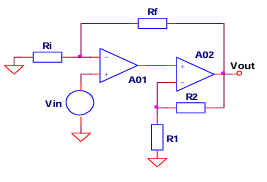
\includegraphics[width=3.04514in,height=2.075in]{media/image1.png}
    \caption{Circuito del amplificador compuesto}
    \label{fig:1}
\end{figure}

La consigna nos indica los requerimientos:

\begin{itemize}
\item
  A\textsubscript{vf} = 20dB
\item
  Máxima planicidad de módulo
\item
  M\textsubscript{\ensuremath{\phi}} = 65\ensuremath{^\circ}
\item
  Q\textsubscript{p} = 0,707
\end{itemize}

\subsection{Amplificador VFA - VFA}\label{amplificador-vfa---vfa}

Como amplificador VFA se utilizó el LM324 el cual presenta las
siguientes características de interés:

\begin{itemize}
\item
  A\textsubscript{do} = 100dB
\item
  F\textsubscript{T} = 1MHz
\item
  F\textsubscript{1} = 10Hz
\item
  F\textsubscript{2} = 5,06MHz
\end{itemize}

Comenzando el análisis para el diseño del amplificador, considerando A02
como ideal, se calcula la ganancia de lazo abierto
A\textsubscript{d}(s), la ganancia de lazo T(s) y la ganancia de lazo
cerrado A\textsubscript{vf}(s).

Para calcular la ganancia de lazo abierto, se eligió abrir el lazo de
realimentación como se muestra a continuación:

\begin{figure}[H]
    \centering
    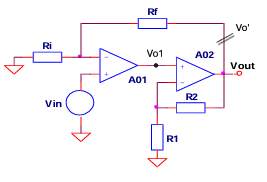
\includegraphics[width=2.78333in,height=1.89653in]{media/image2.png}
    \caption{Corte de lazo de realimentación}
    \label{fig:2}
\end{figure}

\subsubsection{\texorpdfstring{Ganancia a lazo abierto
A\textsubscript{v}(s)}{Ganancia a lazo abierto Av(s)}}\label{ganancia-a-lazo-abierto-avs}

\[A_{v}(s) = \ \left. \ \frac{V_{out}}{V_{in}} \right\rfloor_{V_{o}^{'} = 0}\]

Analizando el circuito

\[V_{o1} = \ A_{d}(s)\ .\ V_{in}\]

\[V_{o} = \ \left( 1 + \ \frac{R_{2}}{R_{1}} \right)\ .\ V_{o1}\]

\[V_{o} = \ \left( 1 + \ \frac{R_{2}}{R_{1}} \right)\ .\ A_{d}(s)\ .\ V_{in}\]

Por lo tanto

\[A_{v}(s) = \ \left( 1 + \ \frac{R_{2}}{R_{1}} \right)\ .\ A_{d}(s)\]

\subsubsection{Ganancia de lazo T(s)}\label{ganancia-de-lazo-ts}

\[T(s) = \ \left. \ \frac{V_{out}}{V_{o}'} \right\rfloor_{V_{in} = 0}\]

\[T(s) = \ \left. \ \frac{V_{o1}}{V_{o}'} \right\rfloor_{V_{in} = 0}.\ \left. \ \frac{V_{out}}{V_{o1}} \right\rfloor_{V_{in} = 0}\]

\[T(s) = \left( - A_{d}(s) \right)\ .\ \left( \frac{R_{i}}{R_{i} + \ R_{f}} \right)\ .\ \left( 1 + \ \frac{R_{2}}{R_{1}} \right)\]

\subsubsection{\texorpdfstring{Ganancia a lazo cerrado
A\textsubscript{vf}(s)}{Ganancia a lazo cerrado Avf(s)}}\label{ganancia-a-lazo-cerrado-avfs}

\[A_{vf}(s) = \ \frac{A_{v}(s)}{1 - \ T(s)}\] \\

Remplazando los resultados obtenidos anteriormente

\[A_{vf}(s) = \ \frac{\left( 1 + \ \frac{R_{2}}{R_{1}} \right)\ .\ A_{d}(s)}{1 + \ \left( A_{d}(s) \right)\ .\ \left( \frac{R_{i}}{R_{i} + \ R_{f}} \right)\ .\ \left( 1 + \ \frac{R_{2}}{R_{1}} \right)}\] \\

Considerando que \(A_{d}(s)\) tiende a ser muy grande, la podemos
considerar como que tiende al infinito para simplificar la expresión, de
forma que nos queda

\[A_{vf}(s) = \ \frac{\left( 1 + \ \frac{R_{2}}{R_{1}} \right)}{\left( \frac{R_{i}}{R_{i} + \ R_{f}} \right)\ .\ \left( 1 + \ \frac{R_{2}}{R_{1}} \right)}\] \\

Por lo tanto

\[A_{vf}(s) = \ \frac{R_{i} + \ R_{f}}{R_{i}}\] \\

Por requerimiento sabemos que \(A_{vf}(s) = 20dB = 10\ veces\), por lo
tanto, podemos definir que

\[\ \frac{R_{i} + \ R_{f}}{R_{i}} = 10\]

Despejando

\[\frac{R_{f}}{R_{i}} = 9\]

Eligiendo valores arbitrarios para las resistencias, cumpliendo con la
condición anterior

\[R_{i} = 1\ K\mathrm{\Omega}\]

\[R_{f} = 9\ K\mathrm{\Omega}\] \\

\subsubsection{\texorpdfstring{Ganancia a lazo cerrado ideal
A\textsubscript{vf2i}(s)}{Ganancia a lazo cerrado ideal Avf2i(s)}}\label{ganancia-a-lazo-cerrado-ideal-avf2is}

El ancho de banda potencia \(f_{g}\) también va a depender de la
ganancia del segundo amplificador A02. Como debemos buscar la condición
de máxima planicidad del módulo, tenemos que:

\[M\varphi = 180{^\circ} - \ {tg}^{- 1}\left( \frac{f_{g}}{f_{1}} \right) - {tg}^{- 1}\left( \frac{f_{g}}{f_{2}} \right)\  = 65,5{^\circ}\]

\newpage

Considerando que

\[f_{g}\  \gg f_{1}\ \  \rightarrow \ {tg}^{- 1}\left( \frac{f_{g}}{f_{1}} \right) = 90{^\circ}\]

Por lo tanto

\[M\varphi = 180{^\circ} - \ 90{^\circ}\  - {tg}^{- 1}\left( \frac{f_{g}}{f_{2}} \right)\  = 65,5{^\circ}\]

\[90{^\circ}\  - {tg}^{- 1}\left( \frac{f_{g}}{f_{2}} \right)\  = 65,5{^\circ}\]

Despejando y resolviendo

\[f_{g} = f_{2}\ .\ tg(24,5{^\circ}) = 2,3\ MHz\] \\

Con este valor podemos calcular la ganancia a lazo cerrado del
amplificador A02 ideal, teniendo en cuenta que \(A_{vfi} = 20\ dB\),
\(A_{d0} = 100\ dB\), y \(\omega_{1} = 2\pi.10\ Hz\ \)

\[A_{vf2i} = \ \frac{A_{vfi}\ .\ \ \omega_{gi}}{{A_{d0}\ .\ \omega}_{1}} = \ \frac{10\ .\ \ 2\pi\ .\ \ 2300000\ Hz}{100000\ .\ 2\pi\ .\ 10\ Hz\ }\]

\[A_{vf2i} = 23\ vez \cong 27\ dB\] \\

Por lo tanto, la ganancia del amplificador compuesto resulta:

\[A_{vcomp} = A_{d0}\ .\ A_{vf2i} = 100000\ .\ 23 = 2300000\ veces \cong 127,2\ dB\]

Con todo esto, finalmente podemos calcular el valor de las resistencias
faltantes

\[A_{vf2i} = \frac{R_{1} + \ R_{2}}{R_{1}} = 23\]

Eligiendo valores arbitrarios para estas resistencias:

\[R_{1} = 22\ K\mathrm{\Omega}\]

\[R_{2} = 1\ K\mathrm{\Omega}\] \\

Ahora, si consideramos el producto (ancho de banda-ganancia) constante,
podemos obtener que:

\[f_{h}\ .\ A_{vf} = A_{do}\ .\ f_{1}\]

\[f_{h}\ .\ 10 = 100000\ .\ 10\ Hz\]

\[f_{h}\  = 100\ KHz\]

Ancho de banda del amplificador compuesto.

\subsubsection{Simulaciones}\label{simulaciones}

Para realizar las simulaciones y comprobar los resultados, se utilizó el
simulador LTspice con las librerías basadas en los datasheets de
National Instruments para los amplificadores operacionales utilizados. \\
Se utilizó el siguiente circuito:
\begin{figure}[H]
    \centering
    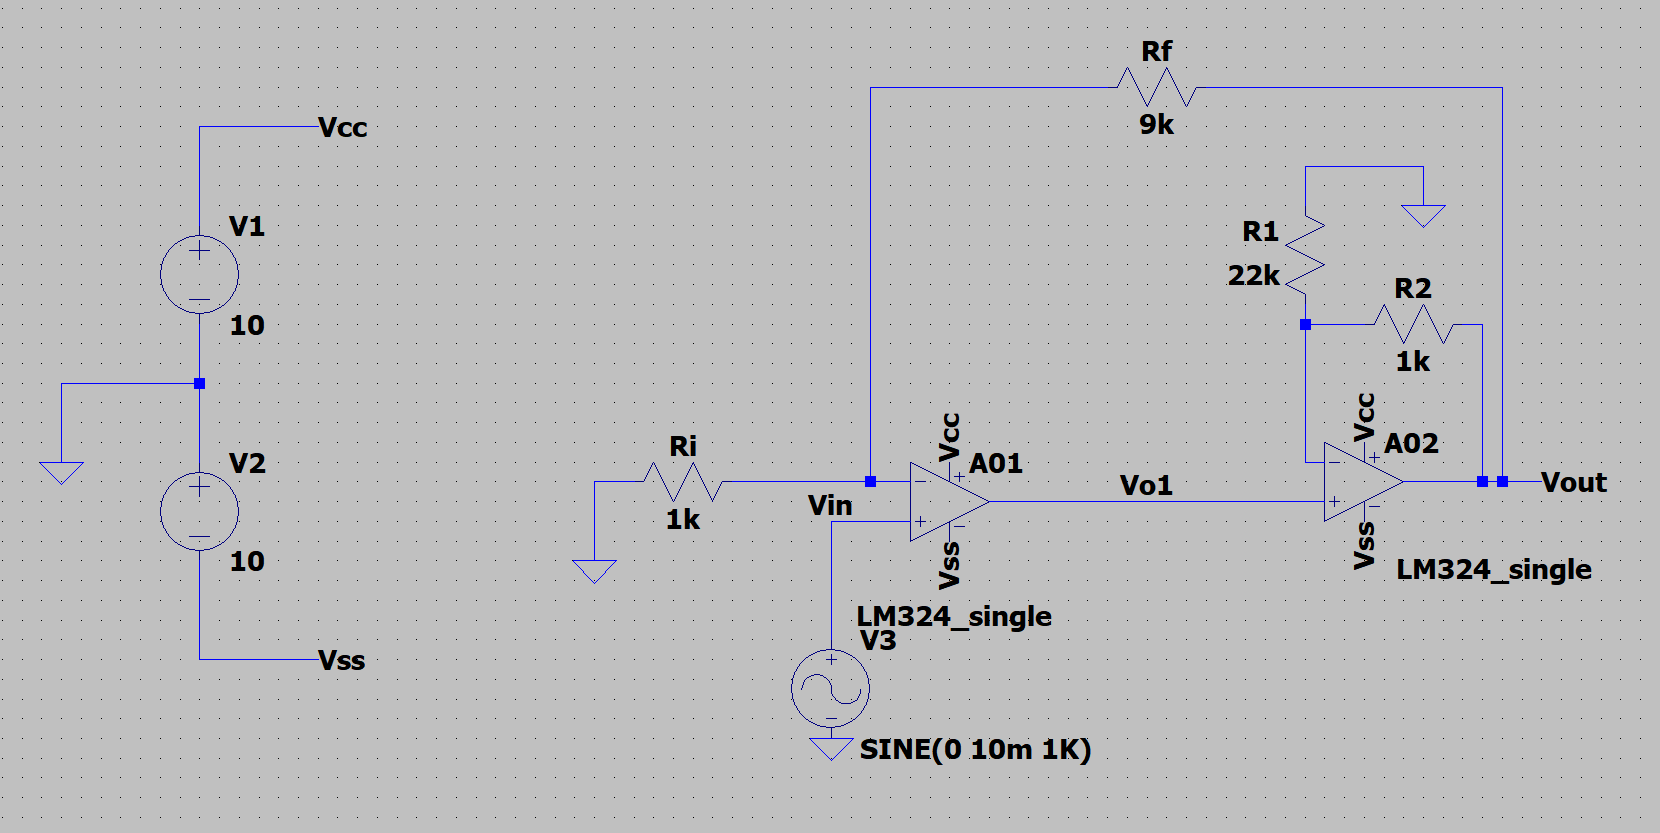
\includegraphics[width=6.1375in,height=3.07986in]{media/image3.png}
      \caption{Circuito para simulación VFA - VFA}
      \label{fig:3}
\end{figure}

En base a este circuito, se realizaron simulaciones para comprobar el
valor de la ganancia del amplificador compuesto y la respuesta en
frecuencia mediante un diagrama de bode realizado por medio de un
barrido en frecuencia.

\begin{figure}[H]
    \centering  
    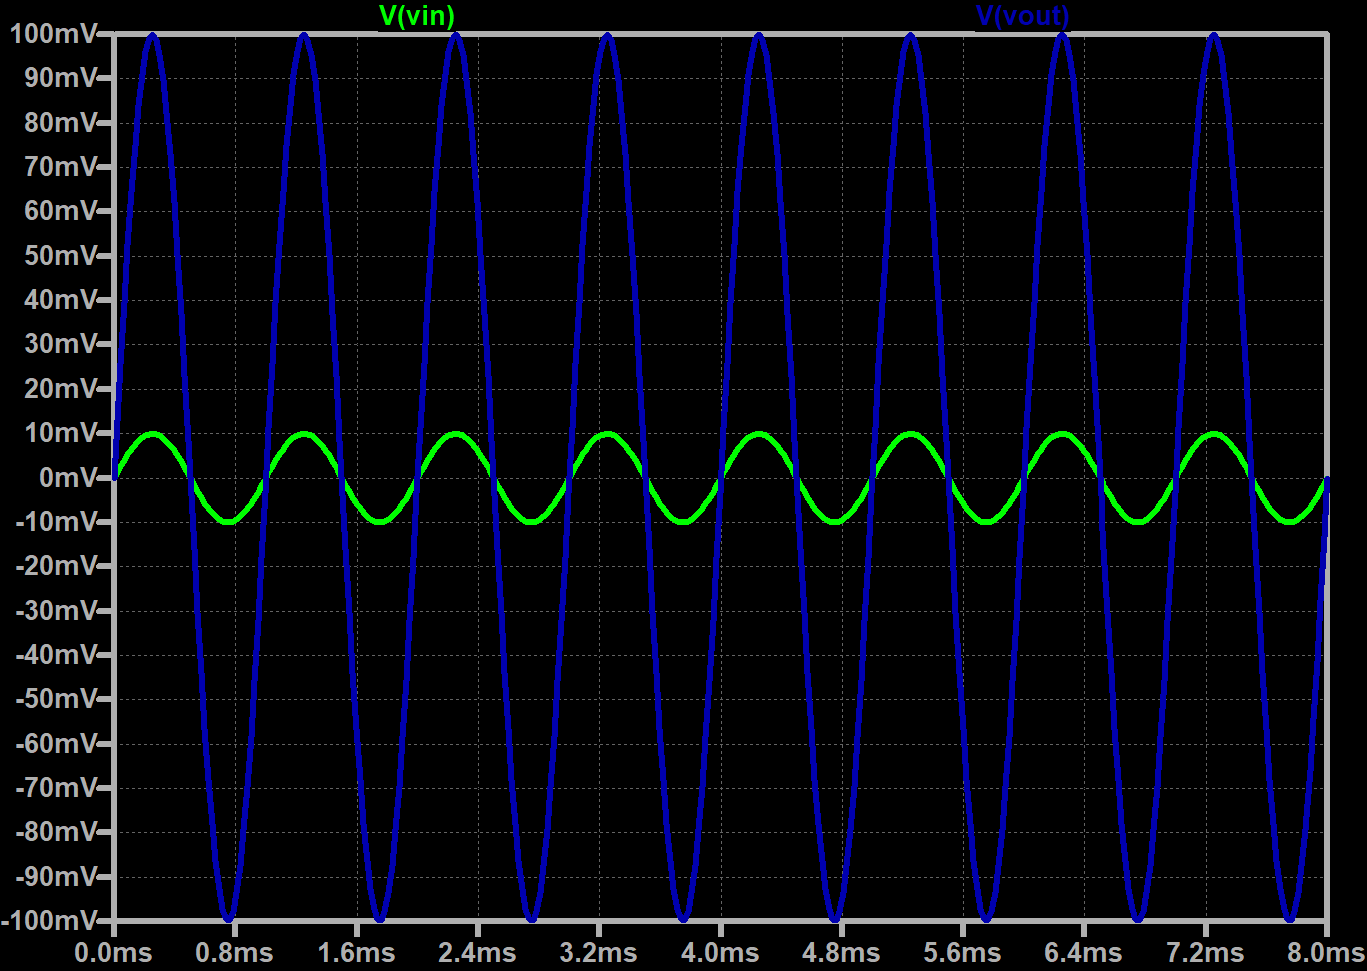
\includegraphics[width=5.21111in,height=3.70139in]{media/image4.png}
    \caption{Ganancia a la salida del sistema VFA-VFA.}
    \label{fig:4}
\end{figure}

\begin{figure}[H]
    \centering
    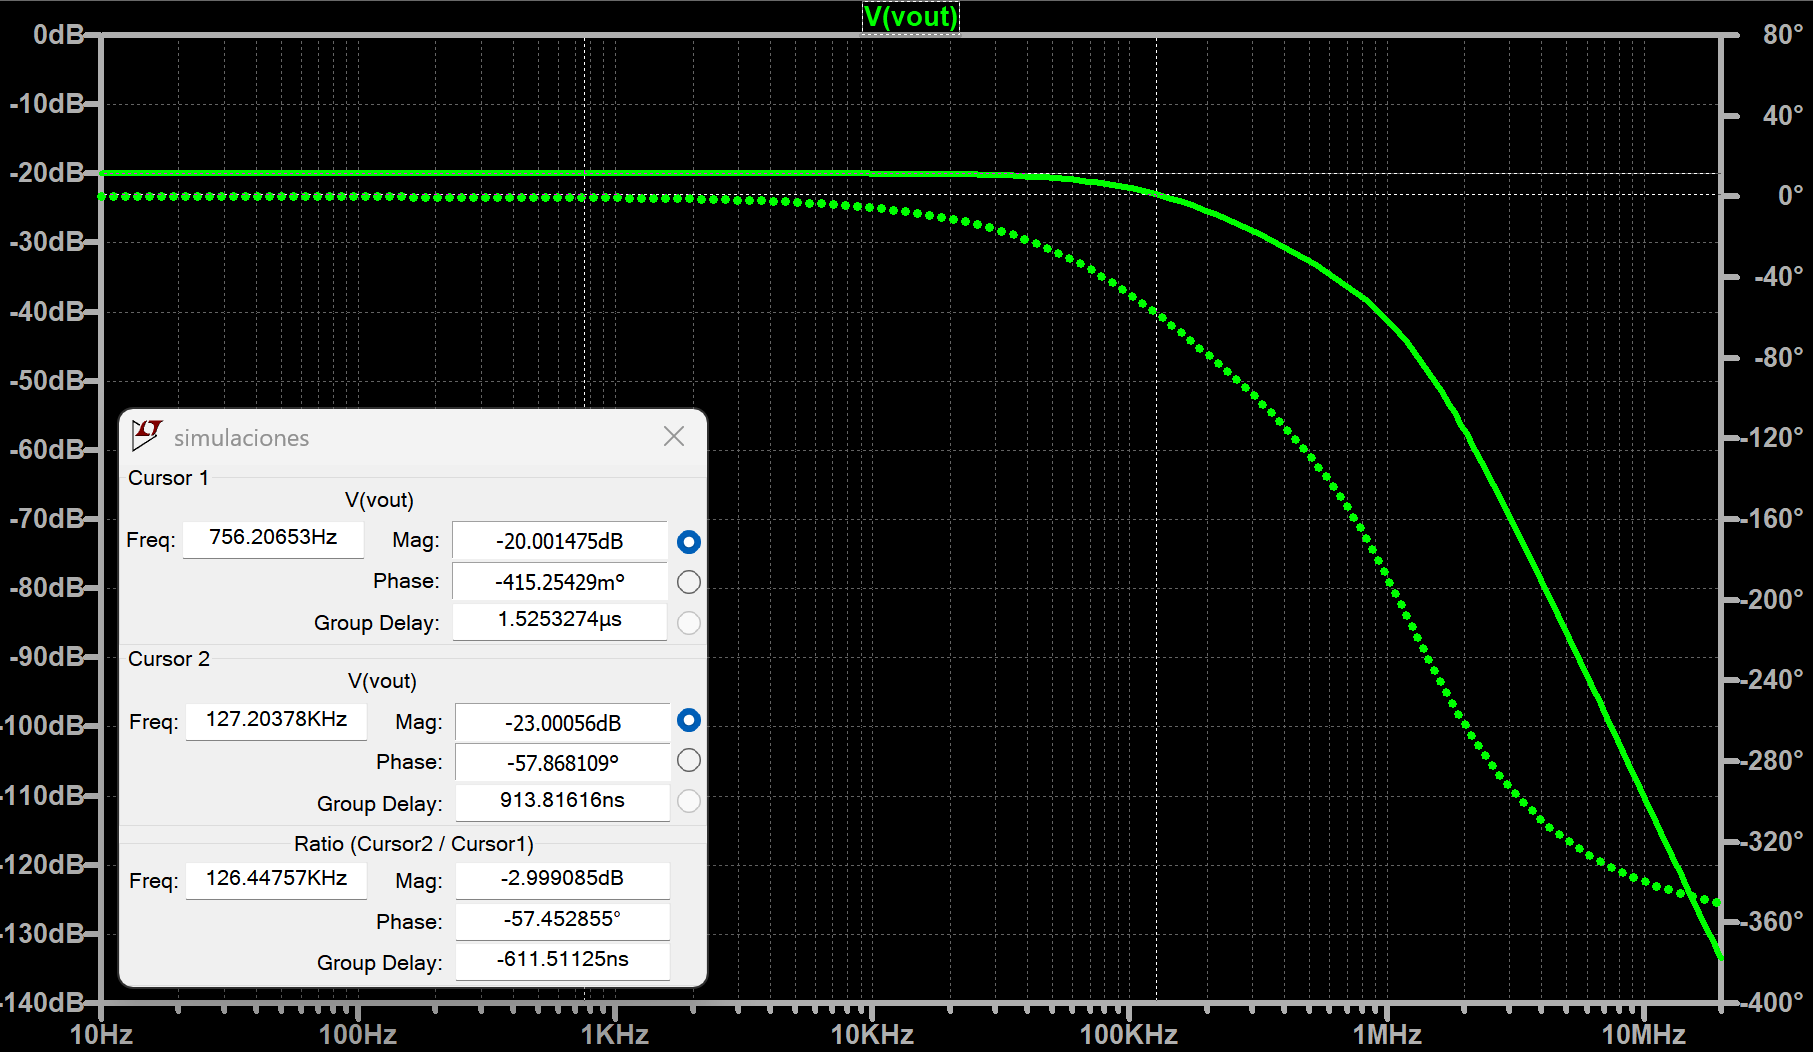
\includegraphics[width=5.2126in,height=3.02446in]{media/image5.png}
    \caption{Respuesta en frecuencia del sistema VFA-VFA.}
    \label{fig:5}
\end{figure}

\subsubsection{Análisis de resultados}\label{anuxe1lisis-de-resultados}

Observando los resultados analíticos y comparándolos con los resultados
de las simulaciones, podemos observar que:

\begin{itemize}
\item
  Ganancia del amplificador compuesto: se observa que los resultados
  analíticos se obtuvieron en base al requerimiento de
  \(A_{vf}(s) = 20dB = 10\ veces\). Ahora, si observamos los resultados
  obtenidos mediante simulación, podemos ver que la ganancia del sistema
  efectivamente vale \(A_{vf}(s)\  \cong 10\ veces\), demostrando que el
  análisis efectuado para el diseño del circuito fue correcto.
\item
  Respuesta en frecuencia: en cuanto al ancho de banda del sistema,
  vemos que los resultados analíticos nos dieron un ancho de banda de
  \(f_{h} = 100\ KHz\). Mediante las simulaciones del sistema, vemos que
  el ancho de banda nos da \(f_{h} = 127\ KHz\). Existe un error entre
  ambos resultados que se puede expresar como:
\end{itemize}

\[E_{\%} = \ \frac{|100 - 127|}{127}\ .\ 100 = 21,2\ \%\]

Este error puede ser debido al modelo paramétrico que utiliza el
simulador para el amplificador LM324.

Aun así, es un error aceptable, por lo tanto, consideramos los
resultados satisfactorios.

\newpage

\subsection{Amplificador VFA - CFA}\label{amplificador-vfa---cfa}

El análisis para este caso se basó en el mismo circuito propuesto en el
caso anterior, remplazando A02 por un CFA.

Como amplificador VFA se utilizó un LM324, al igual que en el caso
anterior, y como amplificador CFA se utilizó un LM6181. Las
características de interés de ambos amplificadores operacionales se
describen a continuación:

\begin{itemize}
\item
  LM324

  \begin{itemize}
  \item
    A\textsubscript{do} = 100dB
  \item
    F\textsubscript{T} = 1MHz
  \item
    F\textsubscript{1} = 10Hz
  \item
    F\textsubscript{2} = 5,06MHz
  \end{itemize}
\item
  LM6181

  \begin{itemize}
  \item
    R\textsubscript{T} = 2,37 M\ensuremath{\Omega}
  \item
    C\textsubscript{T} = 4,8 pF
  \item
    F\textsubscript{1} = 14 KHz
  \item
    F\textsubscript{2} = 82,3 MHz
  \end{itemize}
\end{itemize}

\subsubsection{Consideraciones de VFA}\label{consideraciones-de-vfa}

Para el análisis en este caso, se considera que el operacional VFA
presenta el mismo comportamiento que en el caso anterior, por lo tanto,
los resultados obtenidos se mantienen iguales.

\[A_{vf}(s) = \ 20\ dB\]

\[R_{i} = 1\ K\mathrm{\Omega}\]

\[R_{f} = 9\ K\mathrm{\Omega}\]

\subsubsection{Análisis de CFA}\label{anuxe1lisis-de-cfa}

Analizando las características de ambos operacionales vemos que:

\[f_{2_{VFA}}\  \ll \ f_{2_{CFA}}\]

Por lo tanto, el polo de alta frecuencia del CFA tiene un efecto
despreciable en la ecuación del margen de fase para máxima planicidad.

De esta forma, la ecuación nos queda:

\[M\varphi = 180{^\circ} - \ {tg}^{- 1}\left( \frac{f_{g}}{f_{1_{VFA}}} \right) - {tg}^{- 1}\left( \frac{f_{g}}{f_{2_{VFA}}} \right) - \ {tg}^{- 1}\left( \frac{f_{g}}{f_{1_{CFA}}} \right)\  = 65,5{^\circ}\]

Por requerimiento sabemos que:

\[f_{g} = 2\ MHz\]

Por lo tanto

\[M\varphi = 180{^\circ} - \ {tg}^{- 1}\left( \frac{2\ MHz}{10\ Hz} \right) - {tg}^{- 1}\left( \frac{2\ MHz}{5,06\ MHz} \right) - \ {tg}^{- 1}\left( \frac{2\ MHz}{f_{CFA}} \right)\  = 65,5{^\circ}\]

Donde

\[{tg}^{- 1}\left( \frac{2\ MHz}{10\ Hz} \right)\  \approx 90{^\circ}\]

\[{tg}^{- 1}\left( \frac{2\ MHz}{5,06\ MHz} \right) = 21,56{^\circ}\]

Por lo tanto

\[180{^\circ} - \ 90{^\circ} - 21,56{^\circ} - \ {tg}^{- 1}\left( \frac{2\ MHz}{f_{CFA}} \right)\  = 65,5{^\circ}\]

Despejando

\[f_{CFA}\  = \ \frac{2\ MHz}{tg(2,94)} = 38,94\ MHz\]

Sabiendo que

\[\omega_{CFA} = \ \frac{1}{C_{T}\ .\ \ R_{2}}\]

\[R_{2} = \ \frac{1}{C_{T}\ .\ \ 2\pi\ .\ f_{CFA}}\]

Por lo tanto

\[R_{2} = \ 851\ \mathrm{\Omega}\]

Ahora, si partimos del producto ganancia-ancho de banda:

\[A_{vf}\ .\ f_{g} = \ A_{d0}\ .\ f_{1}\ .\ A_{vf2}\]

Siendo \(A_{vf2}\) la ganancia ideal a lazo cerrado del CFA.

Despejando

\[A_{vf2}\  = \ \frac{A_{vf}\ .\ f_{g}}{A_{d0}\ .\ f_{1}}\]

\[A_{vf2}\  = \ \frac{10\ .\ \ 2\ MHz}{100000\ .\ 10\ Hz}\]

\[A_{vf2}\  = \ 20\]

Analizando el circuito sabemos que

\[A_{vf2}(s) = \ 1 + \frac{R_{2}}{R_{1}}\]

\[R_{1} \cong 45\]

\subsubsection{Simulaciones}\label{simulaciones-1}

Para realizar las simulaciones y comprobar los resultados, se utilizó el
simulador LTspice con las librerías basadas en los datasheets de
National Instruments para los amplificadores operacionales utilizados.

Se utilizó el siguiente circuito:

\begin{figure}[H]
    \centering
    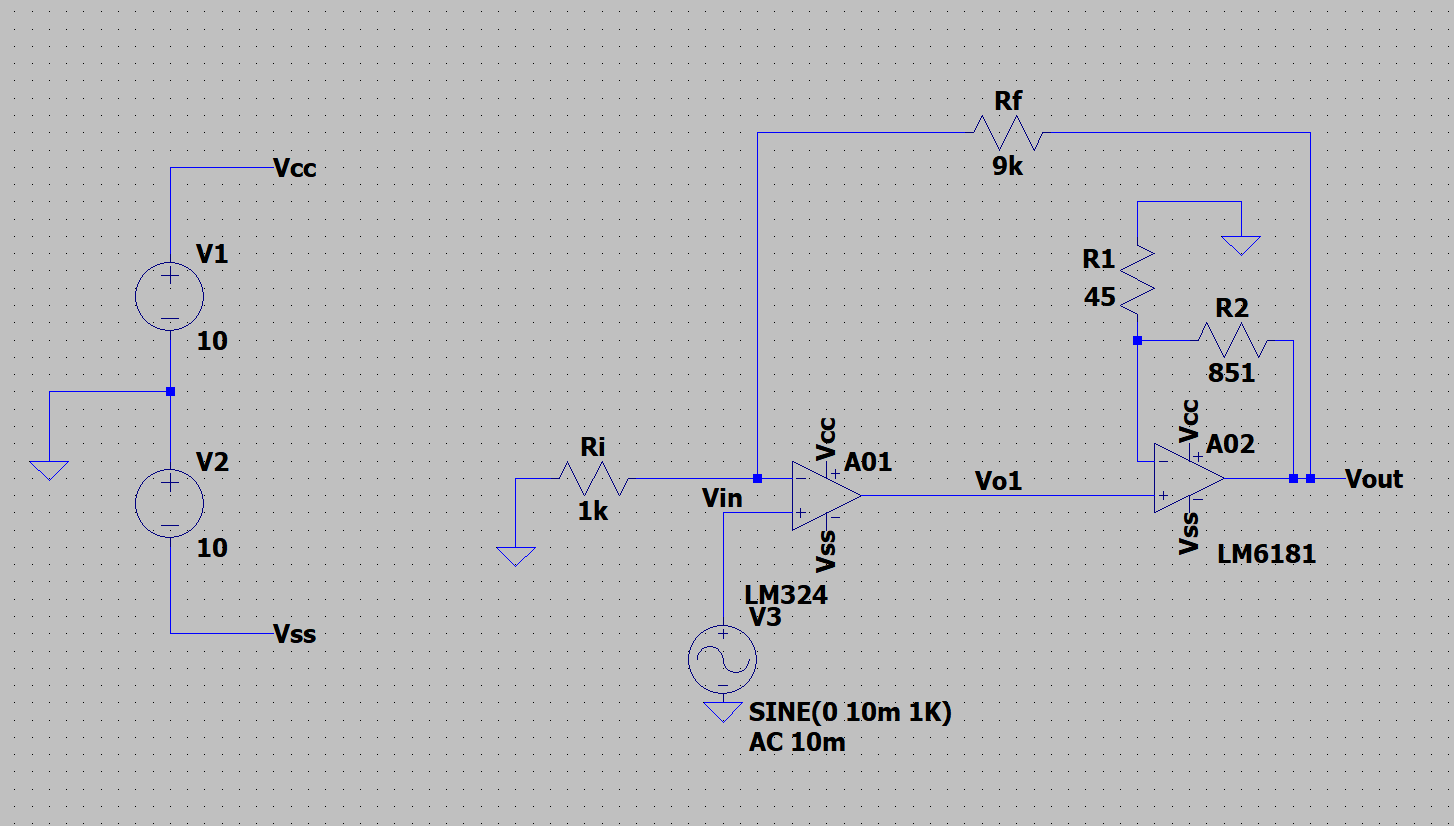
\includegraphics[width=6.1375in,height=3.48611in]{media/image6.png}
    \caption{Circuito para simulación VFA - CFA}
    \label{fig:6}
\end{figure}

En base a este circuito, se realizaron simulaciones para comprobar el
valor de la ganancia del amplificador compuesto y la respuesta en
frecuencia mediante un diagrama de bode realizado por medio de un
barrido en frecuencia.

\begin{figure}[H]
    \centering
    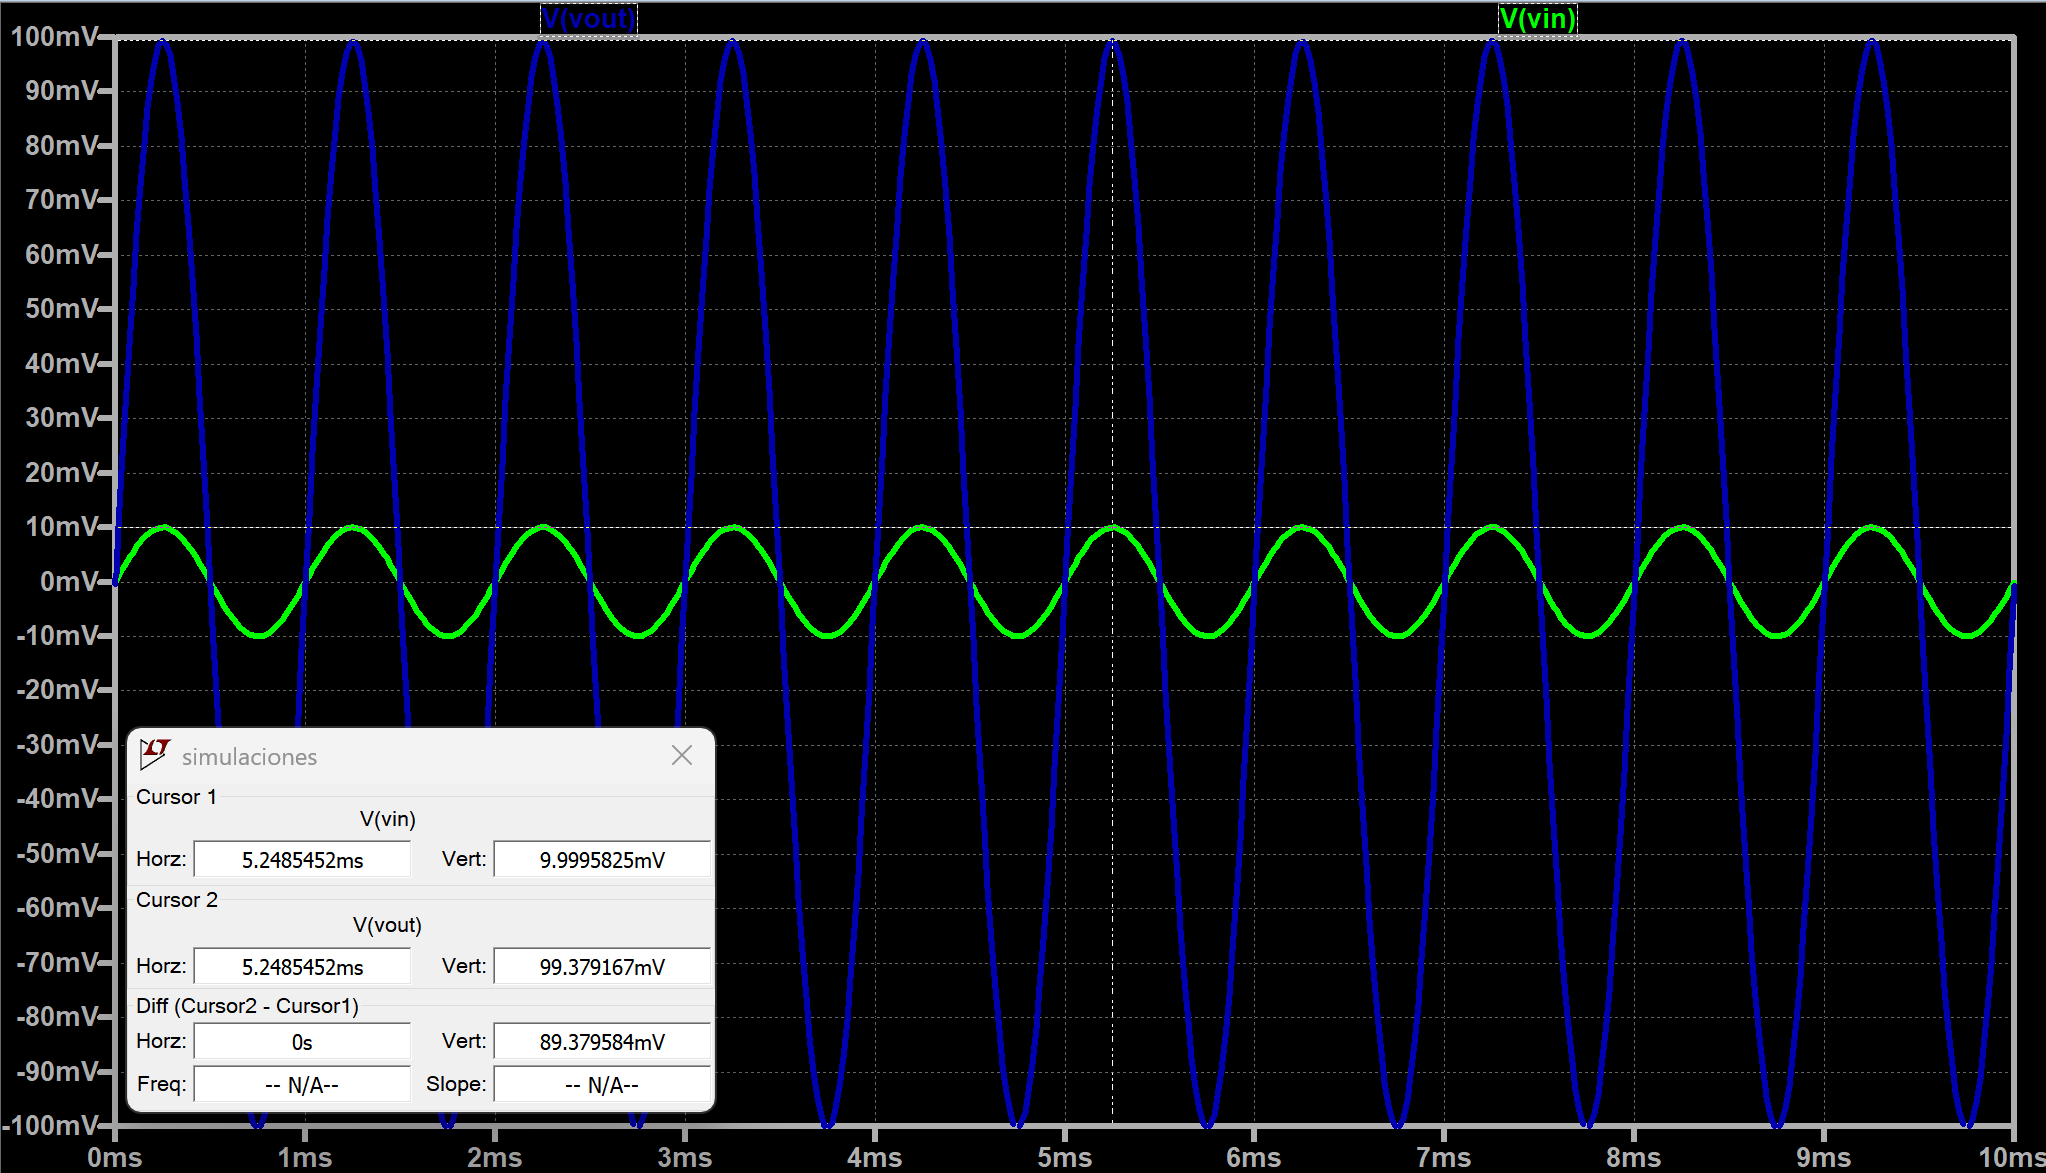
\includegraphics[width=5.2126in,height=2.98849in]{media/image7.png}
    \caption{Ganancia a la salida del sistema VFA-CFA.}
    \label{fig:7}
\end{figure}

\begin{figure}[H]
    \centering
    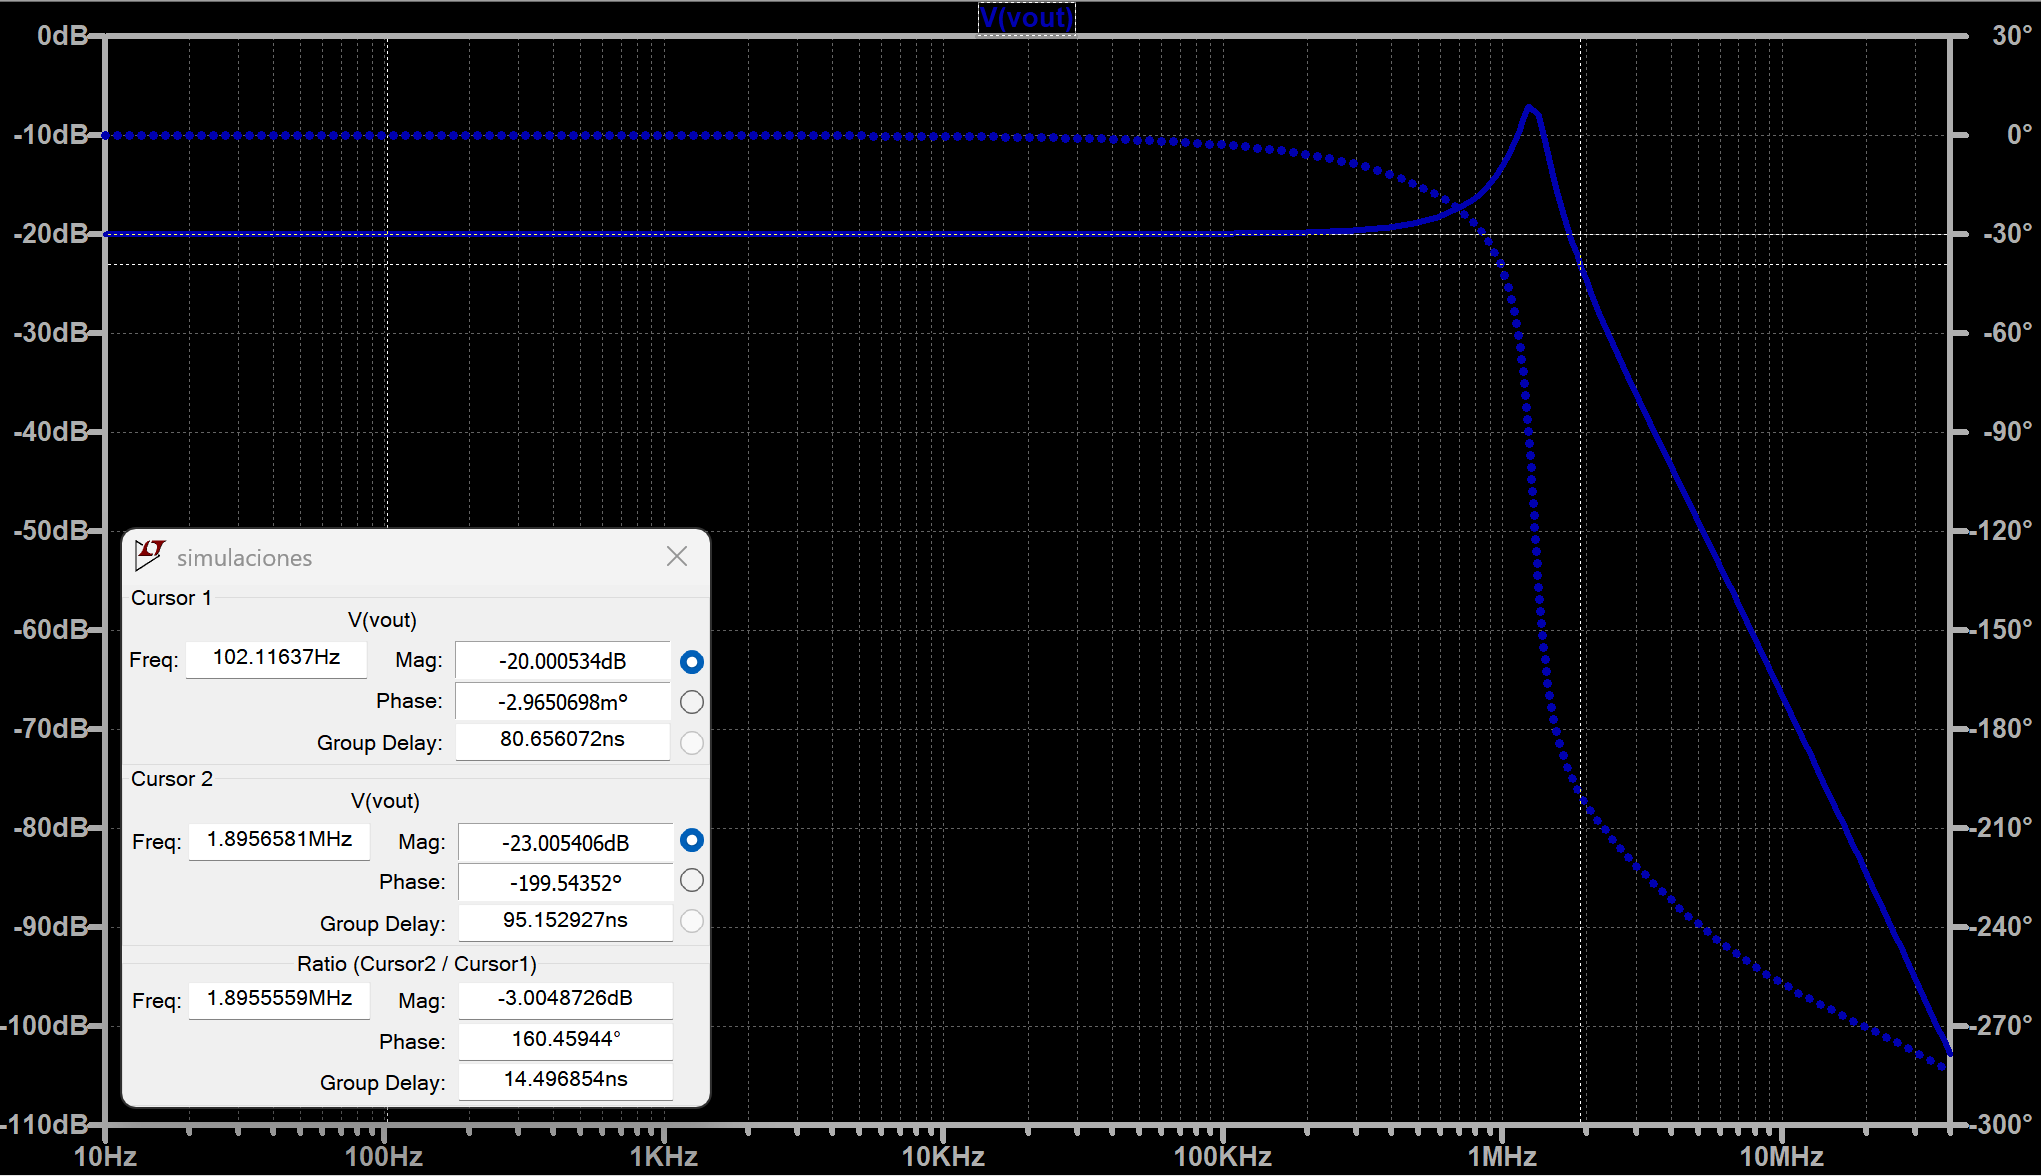
\includegraphics[width=5.2126in,height=3.00323in]{media/image8.png}
    \caption{Respuesta en frecuencia del sistema VFA-CFA.}
    \label{fig:8}
\end{figure}

\subsubsection{Análisis de
resultados}\label{anuxe1lisis-de-resultados-1}

Observando los resultados analíticos y comparándolos con los resultados
de las simulaciones, podemos observar que:

\begin{itemize}
\item
  Ganancia del amplificador compuesto: se observa que los resultados
  analíticos se obtuvieron en base al requerimiento de
  \(A_{vf}(s) = 20dB = 10\ veces\). Como la configuración de A01
  permaneció constante, en este caso, se introdujeron cambios únicamente
  en A02. Si observamos las simulaciones, vemos que la ganancia
  \(A_{vf}(s)\  \cong 10\ veces\), comprobando los cálculos analíticos
  realizados.
\item
  Respuesta en frecuencia: en cuanto al ancho de banda del sistema,
  vemos que, por requerimiento, el ancho de banda potencia debía ser
  \(f_{g} = 2\ MHz\). Realizando la simulación, pudimos observar que el
  ancho de banda nos dio de 1,89 MHz, representando un error porcentual
  de:
\end{itemize}

\[E_{\%} = \ \frac{|2 - 1,89|}{1,89}\ .\ 100 = 5,82\ \%\]

Este error puede ser debido al modelo paramétrico que utiliza el
simulador para el amplificador LM6181.

Aun así, es un error aceptable, por lo tanto, consideramos los
resultados satisfactorios.

\newpage

\subsection{Amplificador VFA -- CFA II}\label{amplificador-vfa-cfa-ii}

En esta sección se pide agregar una red de compensación cero -- polo de
tal modo que el cero de la red cancele el segundo polo del VFA el cual
se ubica en 5,06 MHz y que el polo de la red esté ubicado a una octava
del cero.

\begin{figure}[H]
    \centering
    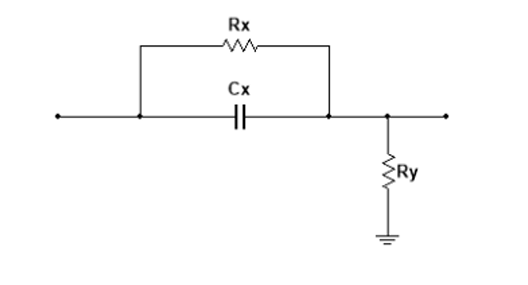
\includegraphics[width=4.26944in,height=2.30417in]{media/image9.png}
    \caption{circuito compensador cero - polo.}
    \label{fig:9}
\end{figure}

\subsubsection{Diseño del compensador cero -
polo}\label{diseuxf1o-del-compensador-cero-polo}

Para comenzar el diseño del compensador requerido, partimos de su
función de transferencia, la cual se expresa de la siguiente forma:

\[A_{c}(s) = \ \frac{R_{y}}{R_{x} + \ R_{y}}\ .\ \frac{1 + {sC_{x}R}_{x}}{1 + {sC_{x}(R}_{x}//R_{y})}\]

Donde podemos definir:

\[k_{comp} = \ \frac{R_{y}}{R_{x} + \ R_{y}}\]

\[\omega_{Pcomp} = \ \frac{1}{1 + {sC_{x}(R}_{x}//R_{y})}\]

\[\omega_{Zcomp} = \ \frac{1}{{C_{x}R}_{x}}\]

Por requerimiento, sabemos que el cero del compensador debe cancelar el
segundo polo del VFA, por lo tanto:

\[\omega_{Zcomp} = \ \frac{1}{{C_{x}R}_{x}} = \ \omega_{2_{VFA}} = 2.\pi.5,06\ MHz\]

Por otro lado:

\[\omega_{Pcomp} = \ \frac{1}{1 + {sC_{x}(R}_{x}//R_{y})} = 2.\omega_{Zcomp} = \ 2.2.\pi.5,06\ MHz = 2.\pi.10,12\ MHz\]

Ahora, si calculamos la ganancia del compensador

\[k_{comp} = \ \frac{\omega_{Zcomp}}{\omega_{Pcomp}} = \ \frac{1}{2} = 0,5\]

Pasando los resultados en limpio

\[k_{comp} = \ 0,5\]

\[\omega_{Pcomp} = \ 2.\pi.10,12\ MHz\]

\[\omega_{Zcomp} = \ 2.\pi.5,06\ MHz\]

Calculado estos valores, podemos pasar a calcular los componentes del
filtro.

Recordando que:

\[k_{comp} = \ \frac{R_{y}}{R_{x} + \ R_{y}} = \frac{1}{2}\]

Despejando

\[R_{x}\  = R_{y}\]

Eligiendo valores arbitrarios

\[R_{x}\  = R_{y} = 1\ K\Omega\]

Calculado el valor de las resistencias, podemos obtener del capacitor
\(C_{x}\) como:

\[\omega_{Zcomp} = \ \frac{1}{{C_{x}R}_{x}} = \ 2.\pi.5,06\ MHz\]

Despejando obtenemos que:

\[C_{x} = \frac{1}{{2.\pi.5,06\ MHz.R}_{x}} = 31\ pF\]

El agregado del compensador trae aparejado una ganancia de
\(k_{comp} = 0,5\), lo cual va a generar que la ganancia del
amplificador compuesto disminuya.

Para compensar este efecto podemos aumentar la ganancia del segundo
amplificador operacional, quedando que:

\[A_{{vf2}_{conp}}(s)\  = 2\ A_{vf2}(s) = 40\ veces\]

Por la tanto, debemos recalcular el valor de las resistencias \(R_{1}\)
y \(R_{2}\).

Recordando que:

\[A_{{vf2}_{conp}} = \frac{R_{1} + \ R_{2}}{R_{1}} = 40\]

Como el polo del CFA permanece invariable

\[R_{2} = 851\]

Con lo que podemos despejar el valor de \(R_{1}\) como:

\[R_{1} = \ \frac{R_{2}}{39} = 22\ \Omega\]

\subsubsection{Simulaciones}\label{simulaciones-2}

Para realizar las simulaciones y comprobar los resultados, se utilizó el
simulador LTspice con las librerías basadas en los datasheets de
National Instruments para los amplificadores operacionales utilizados.

Se utilizó el siguiente circuito:

\begin{figure}[H]
    \centering
    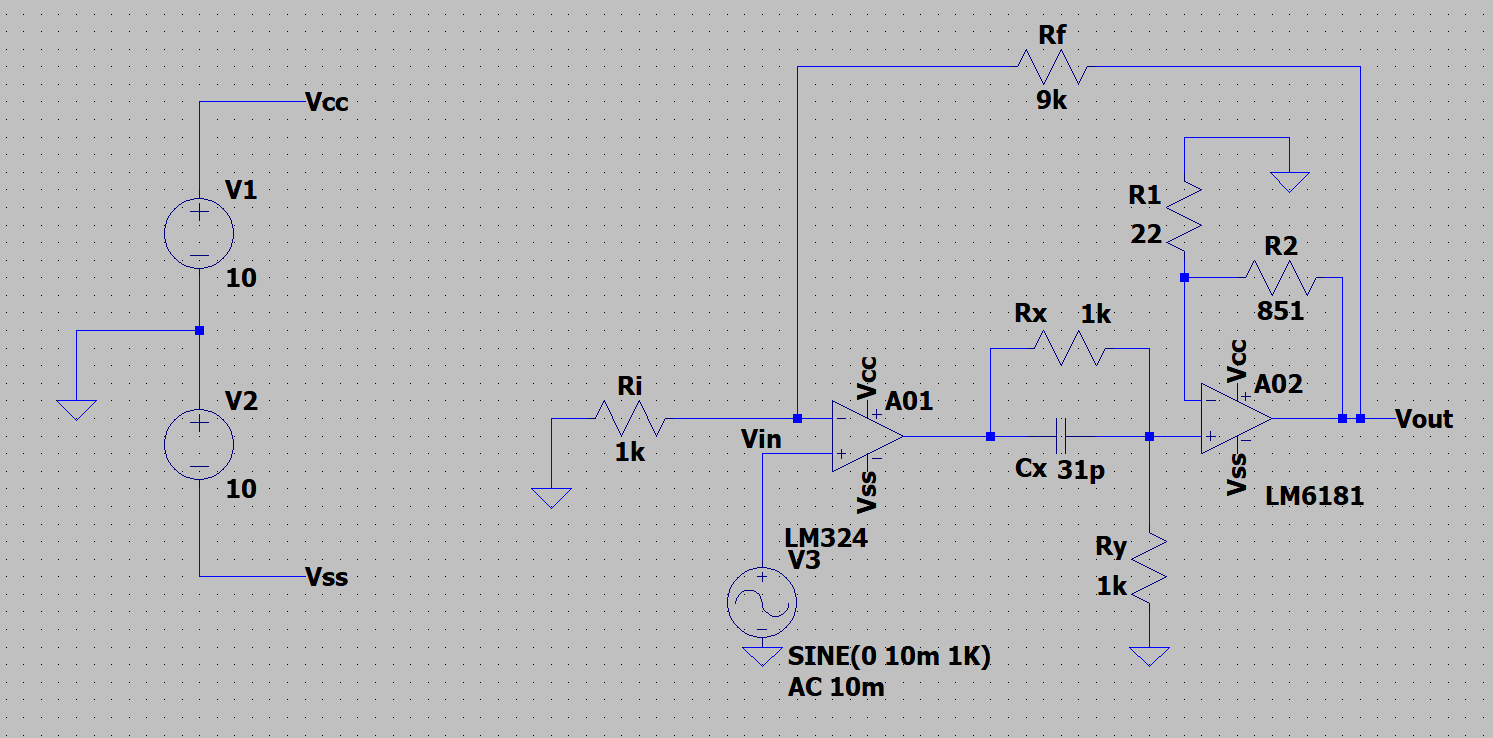
\includegraphics[width=6.1378in,height=3.03348in]{media/image10.png}
    \caption{circuito para simulacion VFA-CFA compensado.}    
    \label{fig:10}
\end{figure}

En base a este circuito, se realizaron simulaciones para comprobar el
valor de la ganancia del amplificador compuesto y la respuesta en
frecuencia mediante un diagrama de bode realizado por medio de un
barrido en frecuencia.

\begin{figure}[H]
    \centering
    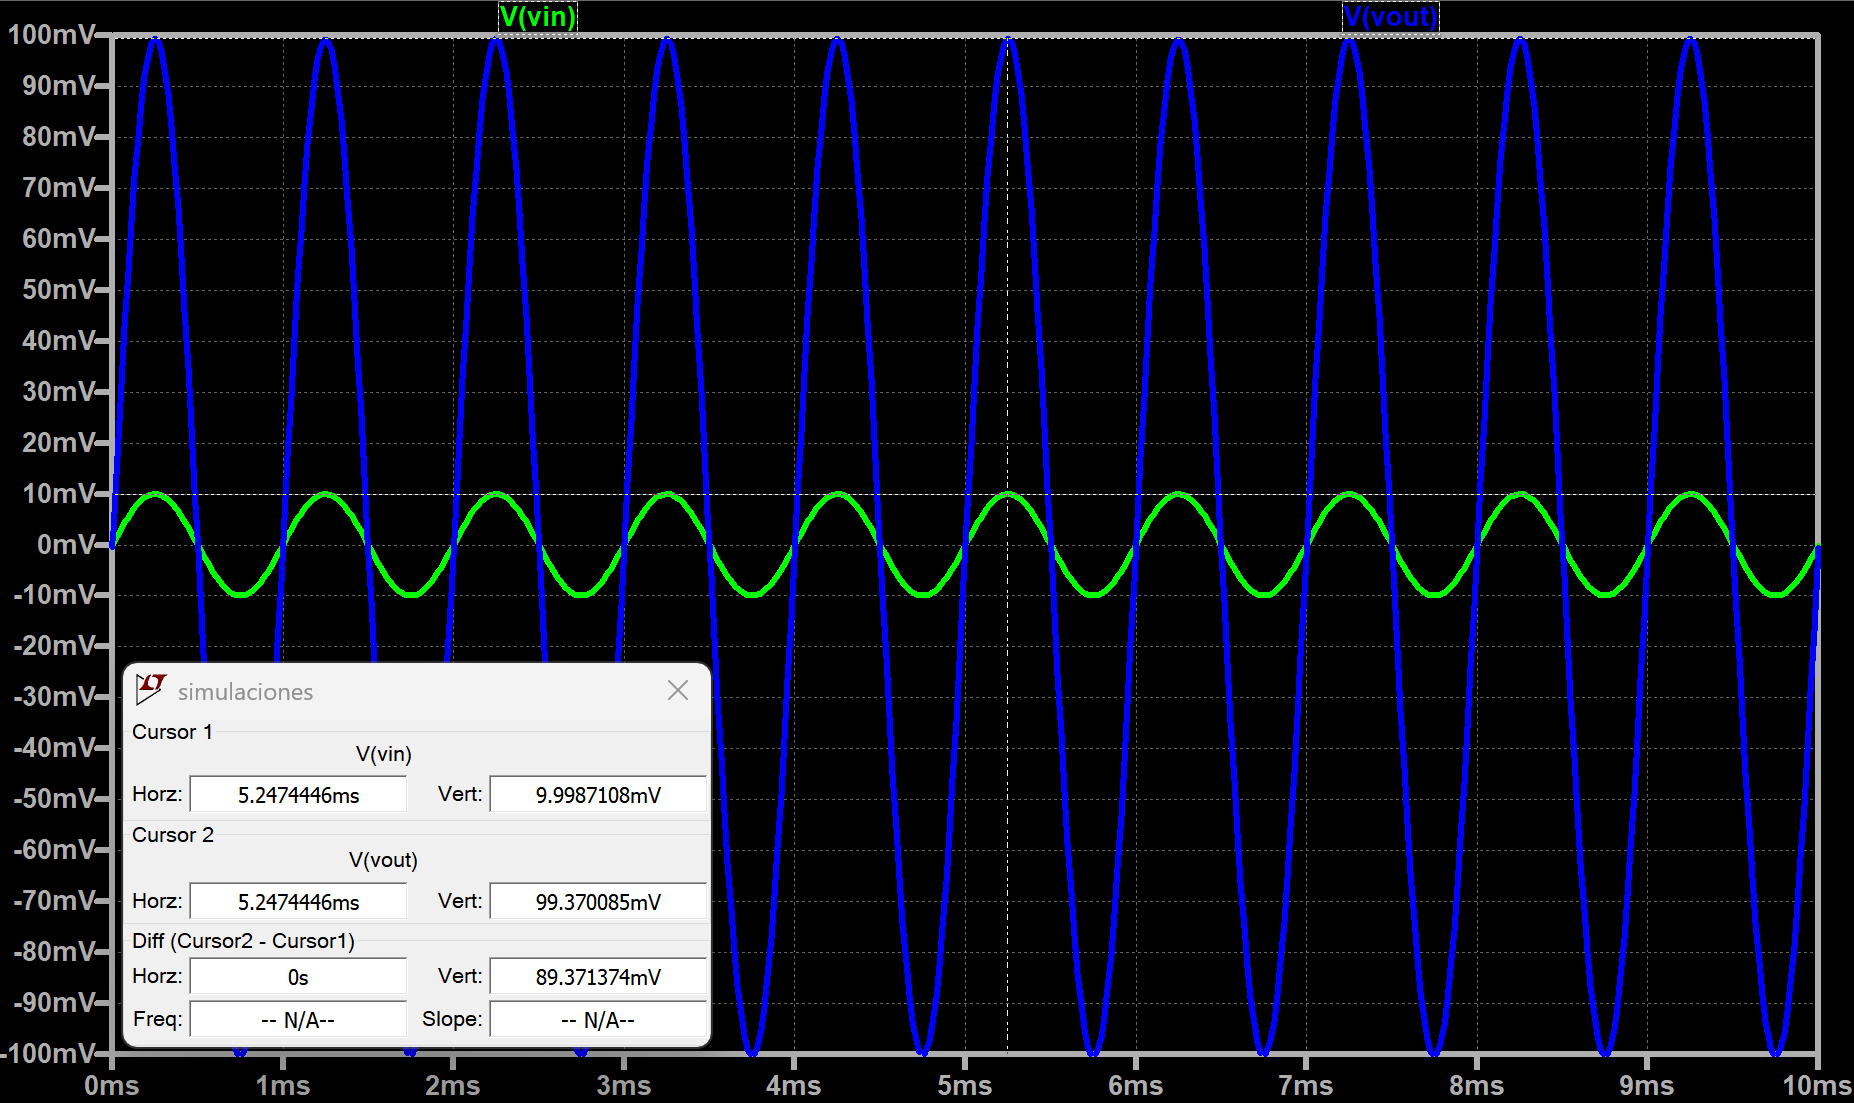
\includegraphics[width=5.2126in,height=3.10114in]{media/image11.png}
    \caption{Ganancia a la salida del sistema VFA-CFA compensado.}
    \label{fig:11}
\end{figure}

\begin{figure}[H]
    \centering
    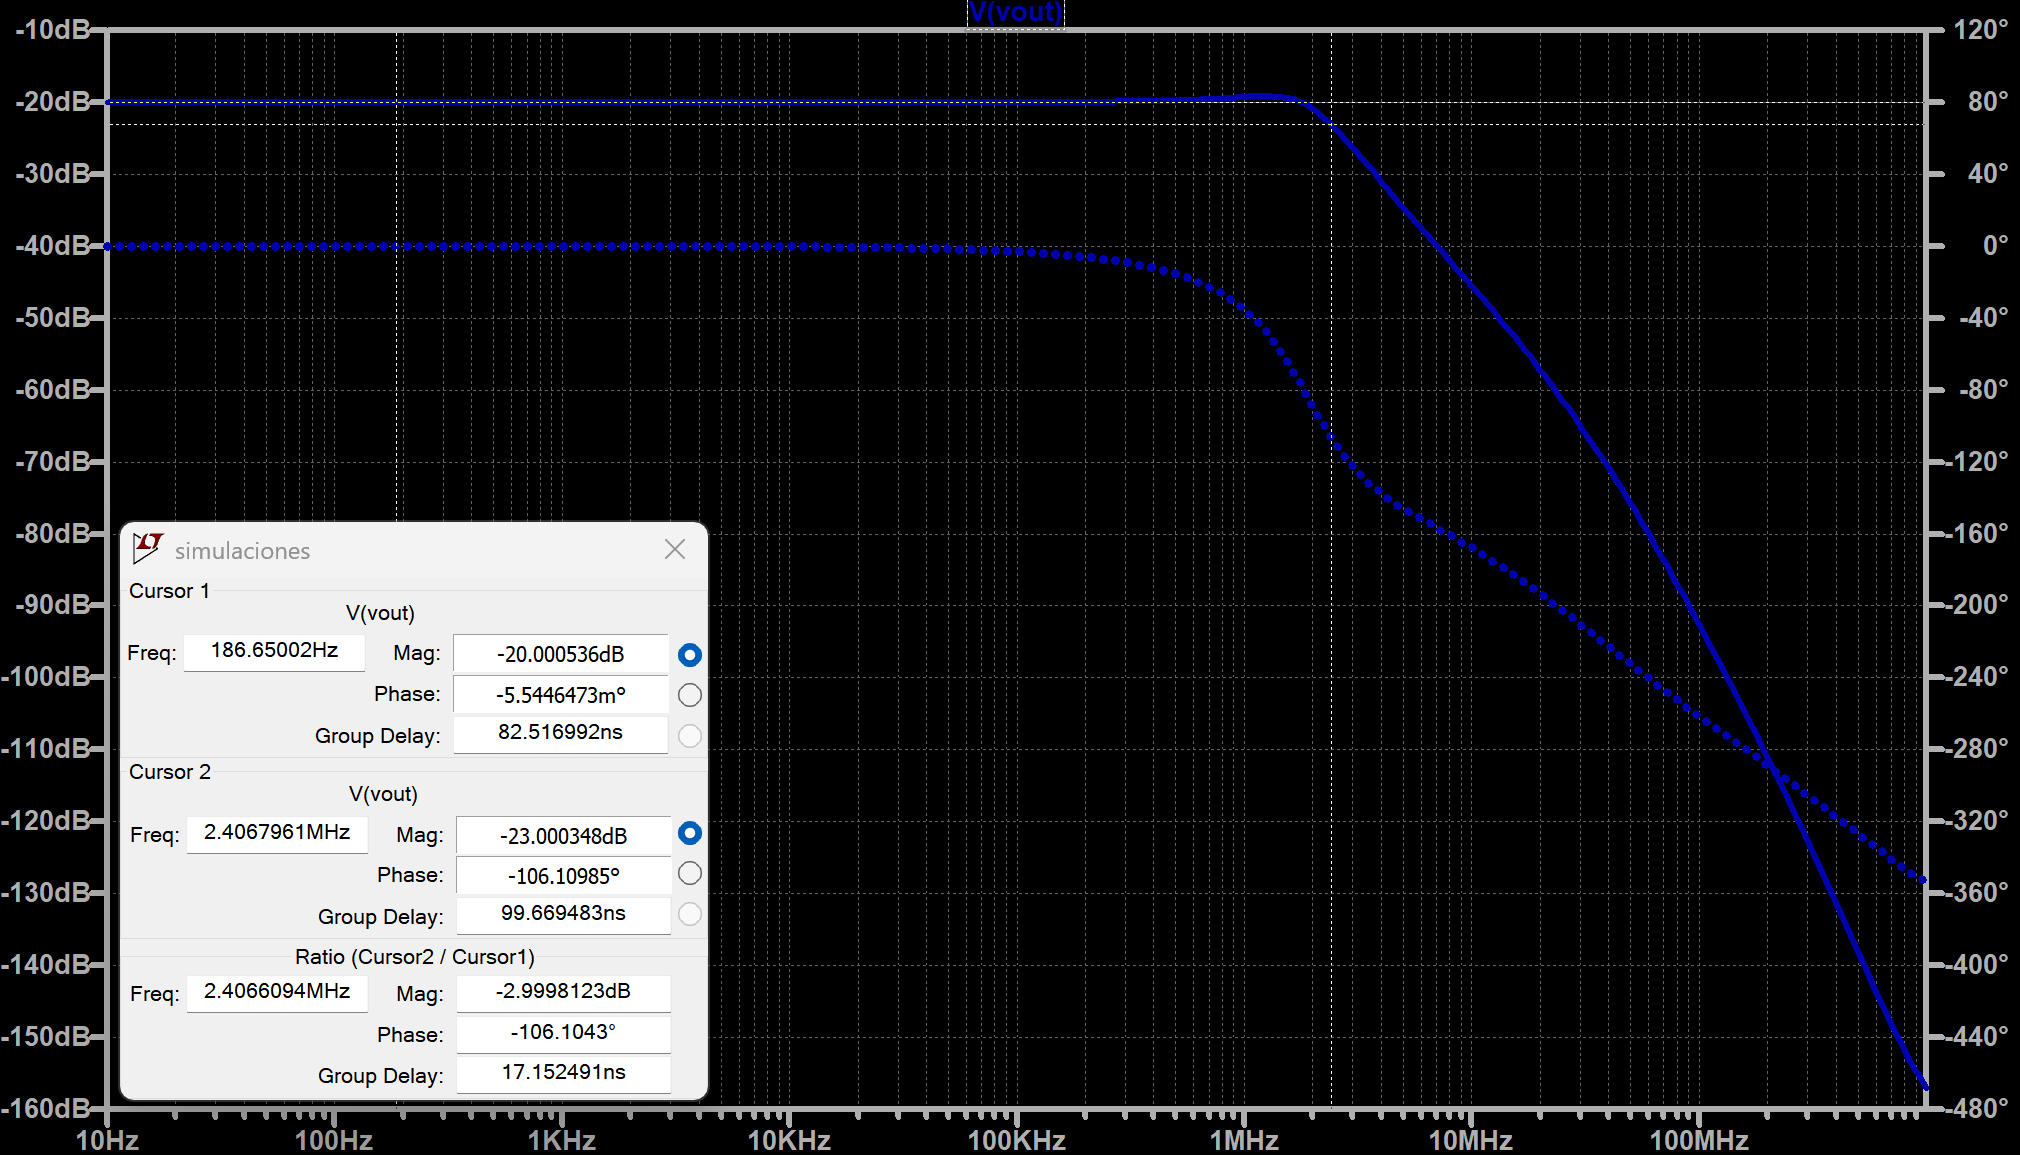
\includegraphics[width=5.2126in,height=2.98023in]{media/image12.png}
    \caption{Respuesta en frecuencia del sistema VFA-CFA compensado.}
    \label{fig:12}
\end{figure}

\subsubsection{Análisis de
resultados}\label{anuxe1lisis-de-resultados-2}

Observando los resultados analíticos y comparándolos con los resultados
de las simulaciones, podemos observar que:

\begin{itemize}
\item
  Ganancia del amplificador compuesto: se observa que los resultados
  analíticos se obtuvieron en base al requerimiento de
  \(A_{vf}(s) = 20dB = 10\ veces\). Al introducir el compensador, vimos
  que el mismo agrega una ganancia de \(k_{comp} = \ 0,5\), lo que
  produce que la ganancia total del sistema disminuya. Por
  requerimiento, la ganancia del sistema debía permanecer constante, por
  lo tanto, se aumentó la ganancia del segundo amplificador para poder
  compensar el efecto de la ganancia del compensador. Realizando las
  simulaciones pudimos comprobar que la ganancia fue compensada
  correctamente, ya que, obtuvimos que \(A_{vf}(s)\  \cong 10\ veces\),
  como se pedía en los requerimientos.
\item
  Respuesta en frecuencia: en cuanto al ancho de banda del sistema,
  vemos que, por requerimiento, el ancho de banda potencia debía ser
  \(f_{g} = 2\ MHz\), al igual que en el caso anterior. Observando los
  resultados de las simulaciones, vemos que la respuesta en frecuencia
  del sistema mejoró, suavizando el pico que se producía en el polo de
  alta frecuencia. Además, pudimos observar un aumento del ancho de
  banda. El nuevo valor de ancho de banda representa un error porcentual
  de:
\end{itemize}

\[E_{\%} = \ \frac{|2 - 2,4|}{2,4}\ .\ 100 = 16,67\ \%\]

El valor es bastante cercano al requerido, por lo que lo podemos
considerar como un error aceptable, por lo tanto, consideramos los
resultados satisfactorios.

\newpage

\section{Conclusión}\label{conclusiuxf3n}

En este trabajo se diseñaron y analizaron amplificadores compuestos utilizando configuraciones VFA-VFA y VFA-CFA, verificando el cumplimiento de las especificaciones establecidas en términos de ganancia, estabilidad y respuesta en frecuencia. A partir del modelado analítico de las funciones de transferencia y del estudio de la ubicación de polos y ceros, se determinaron los valores de los componentes necesarios para obtener una ganancia de 20 dB, máxima planicidad del módulo y un margen de fase cercano a 65°, cumpliendo con los criterios de diseño propuestos. 

Los resultados obtenidos mediante simulaciones en LTspice demostraron el cumplimiento de los valores calculados analíticamente, validando el procedimiento de diseño adoptado. Las diferencias observadas en el ancho de banda se mantuvieron dentro de márgenes aceptables y pueden atribuirse a simplificaciones del modelo teórico y a las aproximaciones empleadas en los modelos de los amplificadores operacionales. En todos los casos se verificó que la respuesta en frecuencia cumple con las condiciones requeridas, manteniendo la estabilidad del sistema. 

La incorporación de la red de compensación cero-polo permitió modificar la respuesta dinámica del sistema, logrando reducir el efecto del polo de alta frecuencia del VFA y mejorar la planicidad del módulo en la zona de transición. Asimismo, se comprobó que la compensación introducida requiere el reajuste de la ganancia del segundo amplificador para mantener el valor especificado de ganancia total. Los resultados obtenidos demuestran que la metodología aplicada permite diseñar amplificadores compuestos que cumplen con las especificaciones planteadas, verificando la validez del análisis teórico mediante simulación. 

\newpage

\section*{Anexo A: Diseño de una Fuente de Tensión CC}

\subsection*{A.1 Topología del circuito}

Se implementa una fuente de tensión continua regulada del tipo \textbf{regulador lineal serie}, compuesta por:

\begin{itemize}
\item Amplificador operacional LM324 como amplificador de error.
\item Transistor BJT NPN (2N3019) como elemento de paso.
\item Referencia de tensión de precisión de $2.5,\mathrm{V}$ (LT1004-2.5 o TL431).
\item Red de realimentación resistiva.
\end{itemize}

El sistema funciona mediante realimentación negativa, comparando una fracción de la tensión de salida con una referencia fija.

\begin{figure}[H]
    \centering
    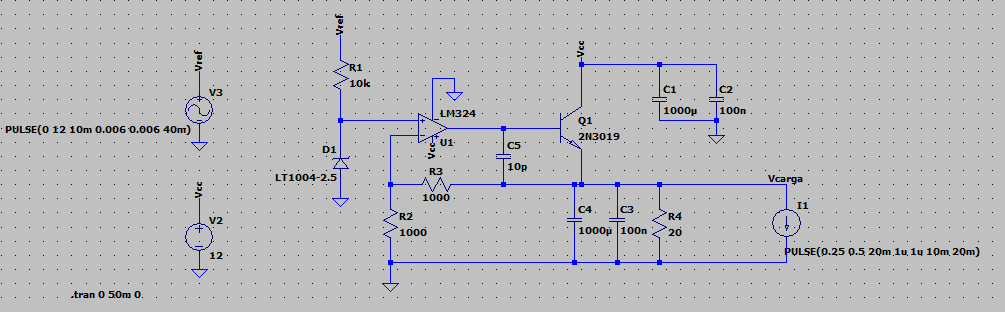
\includegraphics[width=0.9\textwidth]{media/Cir_Fuente_sim.png}
    \caption{Esquema de la fuente de tensión diseñada}
    \label{fig:fuente}
\end{figure}

\subsection*{A.2 Cálculo de la tensión de salida}

La tensión de salida queda definida por:

\[
V_{out} = V_{ref} \left(1 + \frac{R_2}{R_1} \right)
\]

Dado:

\[
V_{ref} = 2.5\,V \quad ; \quad V_{out} = 5\,V
\]

Se obtiene:

\[
5 = 2.5 \left(1 + \frac{R_2}{R_1} \right)
\Rightarrow \frac{R_2}{R_1} = 1
\]

Por lo tanto, se selecciona:

\[
R_1 = R_2 = 1\,k\Omega
\]

Para mejorar la precisión (tolerancia $\pm 0.1,\mathrm{V}$), se recomienda utilizar resistencias de $1\%$.

\subsection*{A.3 Análisis de potencia en el transistor}

El transistor de paso disipa potencia debido a la caída de tensión:

\[
P = (V_{\mathrm{in}} - V_{\mathrm{out}})\cdot I_{\mathrm{out}}
\]

\[
P = (12\mathrm{V} - 5\mathrm{V}) \cdot 0.5\mathrm{A} = 3.5\mathrm{W}
\]

Por lo tanto, es necesario el uso de un disipador térmico para garantizar operación segura.

\subsection*{A.4 Dimensionamiento de capacitores de filtrado}

\subsubsection*{Capacitor de entrada}

Se incorpora un capacitor para reducir el ripple de la fuente de entrada:

\begin{itemize}
\item $C_{\mathrm{in}} = 470,\mu\mathrm{F}$ (electrolítico)
\item $C_{\mathrm{in2}} = 100,\mathrm{nF}$ (cerámico)
\end{itemize}

\subsubsection*{Capacitor de salida}

Para cumplir con la especificación de ripple menor al $1\%$ de la tensión de salida:

\[
\Delta V_{\mathrm{max}} = 0.01 \cdot 5,\mathrm{V} = 50,\mathrm{mV}
\]

El capacitor de salida mejora la respuesta ante cambios de carga y reduce el rizado:

\begin{itemize}
\item $C_{\mathrm{out}} = 470,\mu\mathrm{F} \text{ a } 1000,\mu\mathrm{F}$
\item $C_{\mathrm{out2}} = 100,\mathrm{nF}$
\end{itemize}

\subsection*{A.5 Compensación del lazo de control}

Debido a la presencia de polos introducidos por el transistor, la carga y el capacitor de salida, se agrega un capacitor de compensación:

\[
C_{\mathrm{comp}} = 10,\mathrm{pF} \text{ a } 100,\mathrm{pF}
\]

Este se conecta entre la salida del amplificador operacional y la entrada inversora.

\subsection*{A.6 Resistencia de base}

Para limitar la corriente de base:

\[
R_b = 100,\Omega \text{ a } 1,\mathrm{k}\Omega
\]

\subsection{Simulaciones}

Se realizaron simulaciones en LTspice para verificar la estabilidad, el ripple y la respuesta dinámica de la fuente.

\begin{figure}[H]
    \centering
    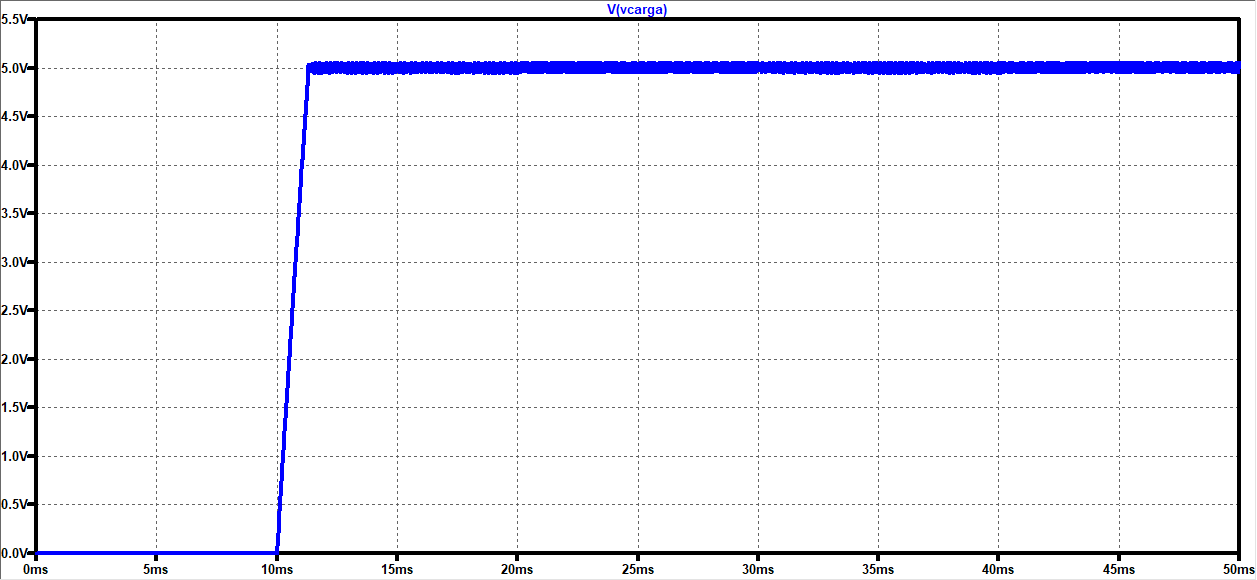
\includegraphics[width=0.7\textwidth]{media/Salida_fuente_sim.png}
    \caption{Respuesta de la fuente de tensión diseñada}
    \label{fig:salida_fuente}
\end{figure}

\begin{figure}[H]
    \centering
    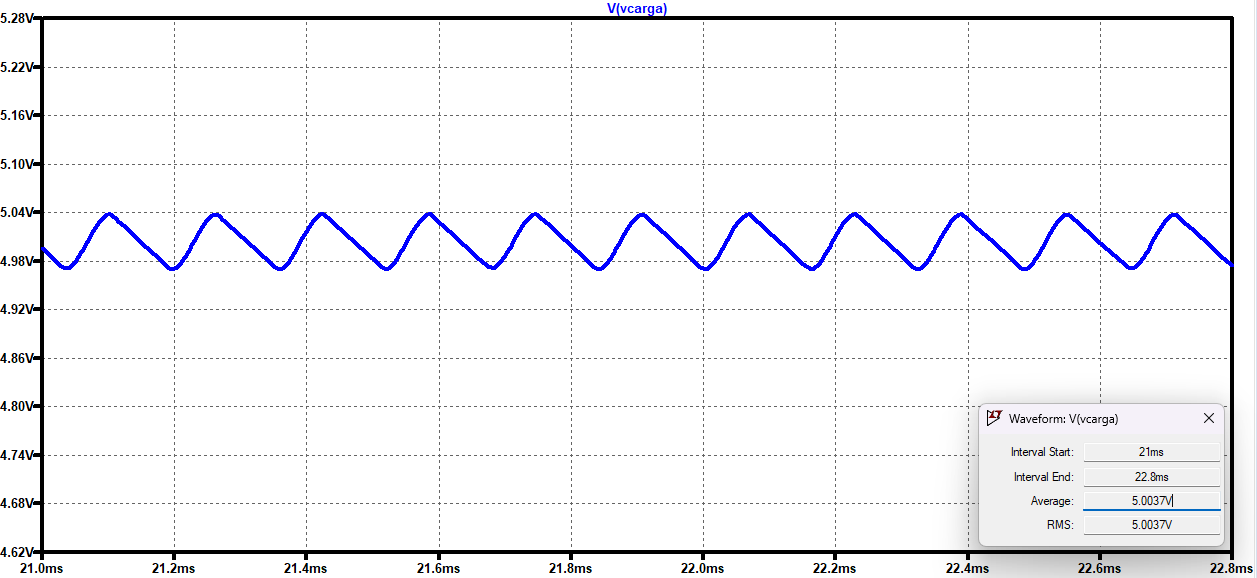
\includegraphics[width=0.7\textwidth]{media/Ripple_fuente_sim.png}
    \caption{Ripple de la fuente de tensión diseñada}
    \label{fig:ripple_fuente}
\end{figure}

Vemos que, a pesar de la variación de carga, la tensión de salida se mantiene estable en $5\mathrm{V}$, con un ripple inferior a $50\mathrm{mV}$, cumpliendo con las especificaciones.

Por otro lado, se midió el valor medio de la tensión de salida, obteniendo un valor de $5.003\mathrm{V}$, por lo que se cumple con los requerimientos planteados en la consigna.

\subsection*{A.8 Conclusión}

A partir del diseño propuesto y la incorporación de los elementos de filtrado, compensación y control, se obtuvo una fuente de tensión lineal regulada capaz de cumplir con las especificaciones establecidas.

El análisis teórico permitió dimensionar adecuadamente la red de realimentación, garantizando una tensión de salida de $5\mathrm{V}$, mientras que el estudio de potencia evidenció la necesidad de disipación térmica en el transistor de paso.

Las simulaciones realizadas en LTspice validan el comportamiento del circuito, observándose que, ante variaciones abruptas de carga entre $250\mathrm{mA}$ y $500\mathrm{mA}$, la tensión de salida se mantiene dentro de los márgenes requeridos. Asimismo, el ripple obtenido resulta inferior a $50\mathrm{mV}$, cumpliendo con la restricción del $1\%$.

Finalmente, el valor medio de salida de $5.003\mathrm{V}$ confirma que el diseño satisface la tolerancia de regulación especificada, evidenciando un funcionamiento estable y robusto frente a perturbaciones dinámicas.

En conjunto, el circuito diseñado cumple con los requisitos de regulación, estabilidad y respuesta dinámica, constituyendo una solución adecuada para una fuente de $5\mathrm{V}$ y $500 \mathrm{mA}$ basada en un regulador lineal serie.

\end{document}
